\section{Identification du grillage}
\begin{frame}{Hypothèses}
\begin{itemize}
	\item Directions du grillage approximativement perpendiculaires (90°$\pm$ 30°)
	\item Lignes dans la transformée de Hough	
\end{itemize}
\begin{figure}[t]
\begin{center}
\begin{tabular}{cccc}
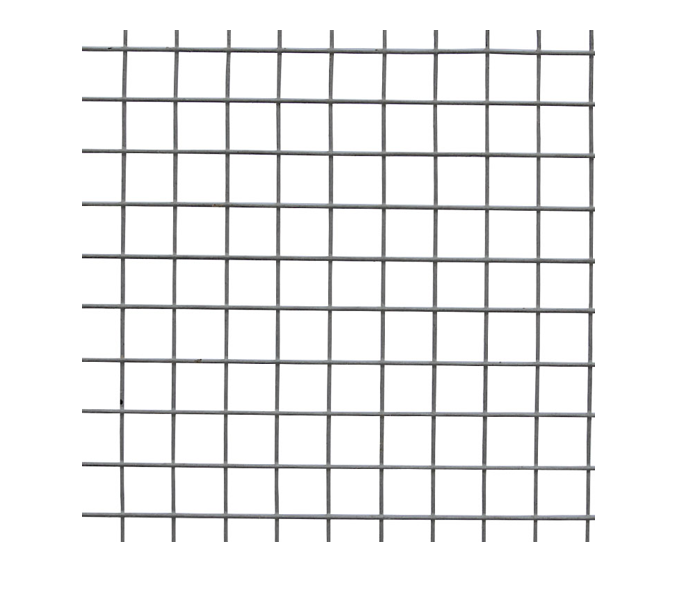
\includegraphics[width = 0.23 \columnwidth]{fig/grillagereduit.png} &
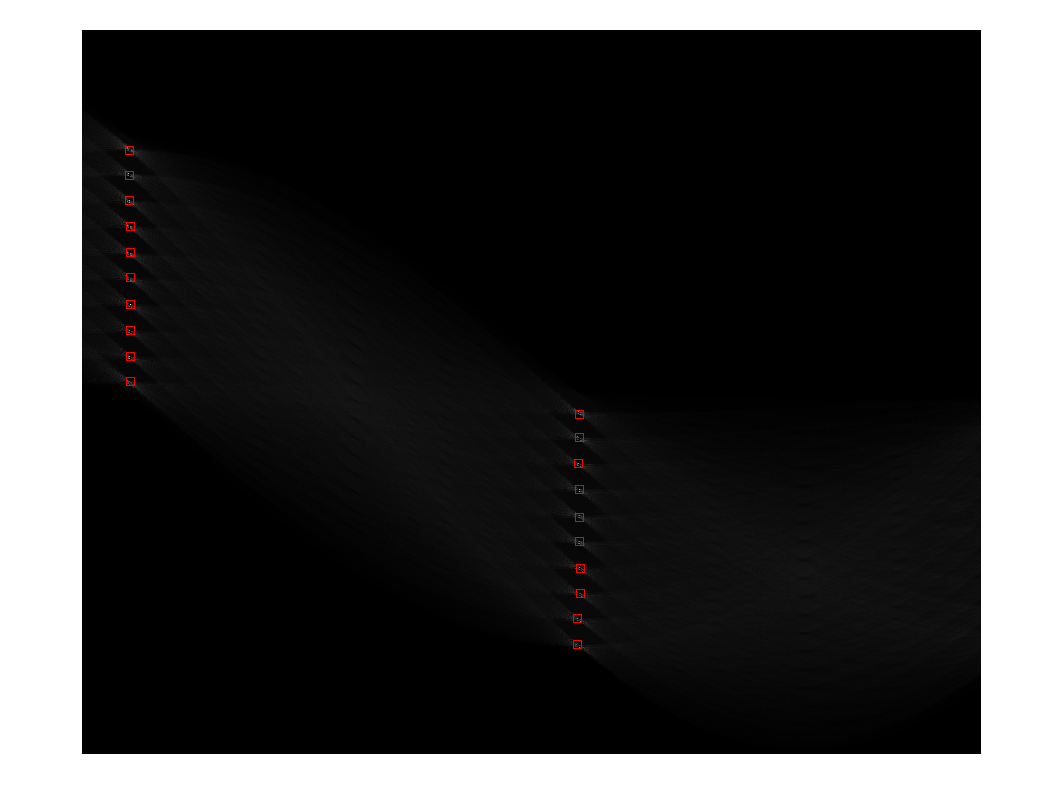
\includegraphics[width = 0.23 \columnwidth]{fig/grillagehough.png}
&
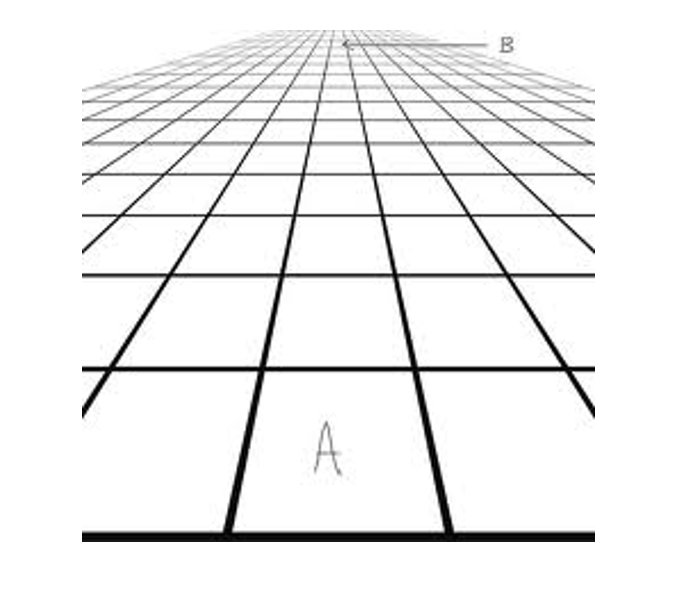
\includegraphics[width = 0.23 \columnwidth]{fig/perspectivereduit.png}
& 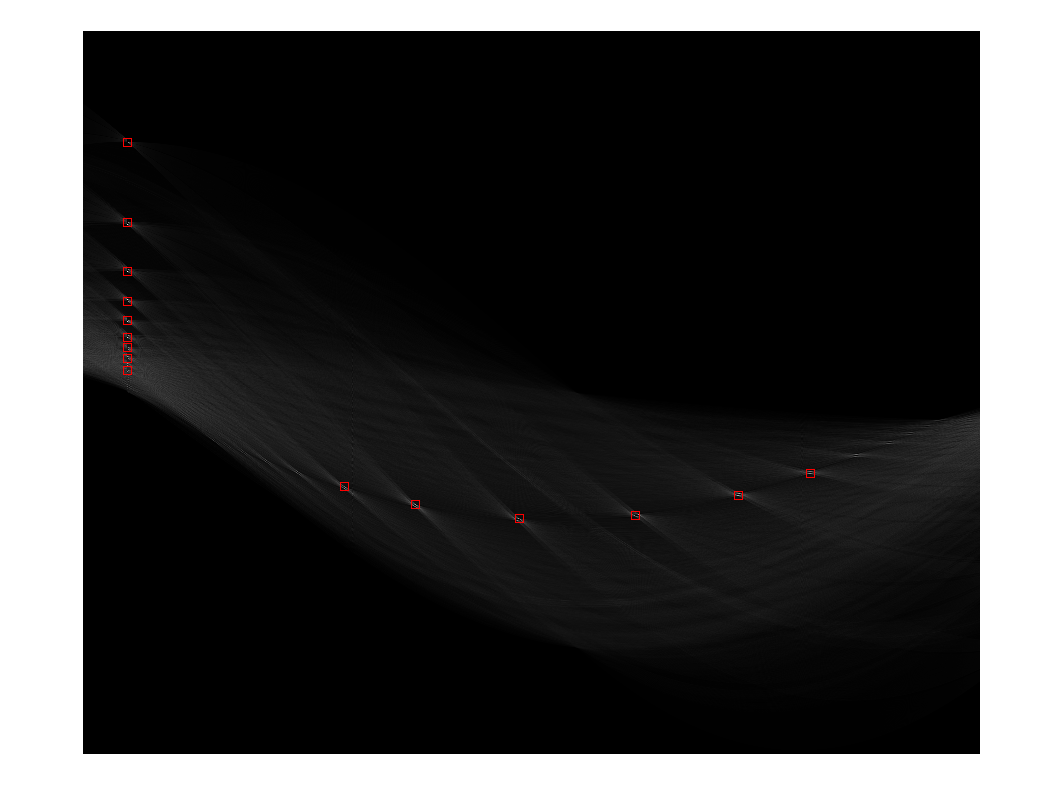
\includegraphics[width = 0.23 \columnwidth]{fig/perspectivehough.png}
\end{tabular}
\caption{\label{houghlines} Illustration de l'impact de la perspective sur les piques troués dans la transformée de Hough}
\end{center}
\end{figure}
\end{frame}

\begin{frame}{Prétraitements}
\begin{itemize}
	\item Centrage de la transformée de Hough
	\item Élimination des artéfacts
\end{itemize}

\begin{figure}[h]
\begin{center}
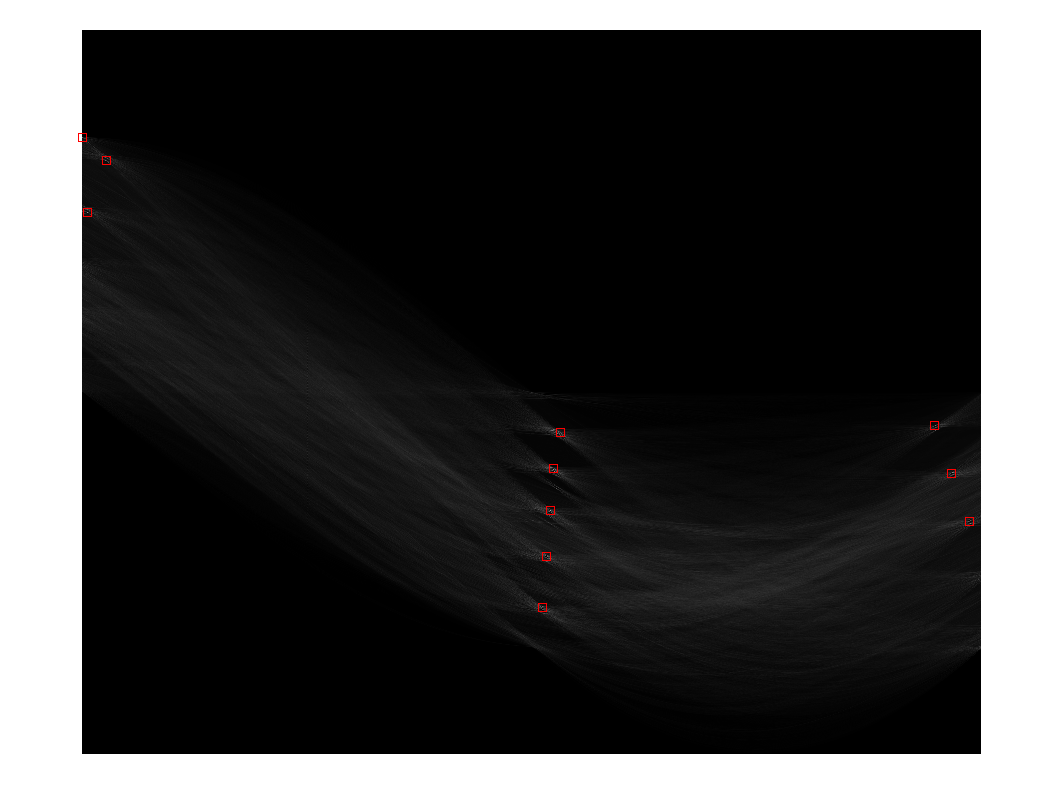
\includegraphics[width = 0.5 \columnwidth]{fig/centrageavt.png}
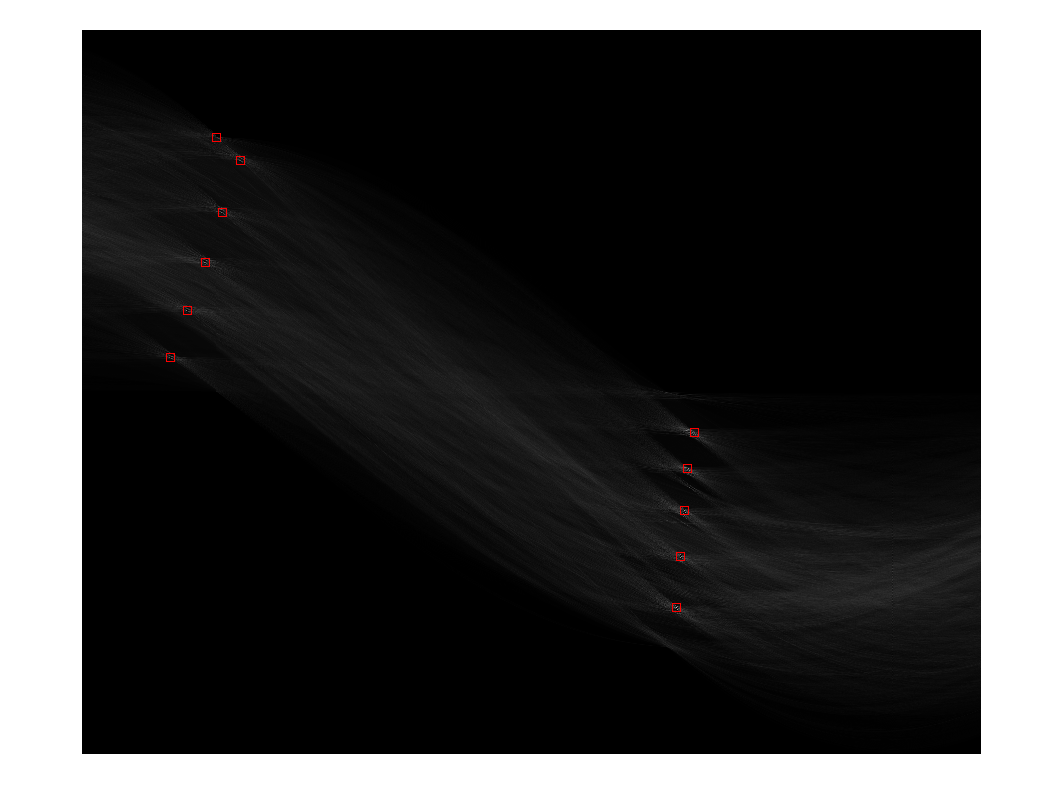
\includegraphics[width = 0.5 \columnwidth]{fig/centrageapres.png}
\caption{\label{centrage} Centrage de la transformée de Hough}
\end{center}
\end{figure}
\end{frame}

\begin{frame}{Détection de lignes dans Hough par Ransac}
\begin{itemize}
\item Essai avec Hough
\item RANSAC sur de larges fenêtres coulissantes
\end{itemize}
\begin{figure}
\begin{center}
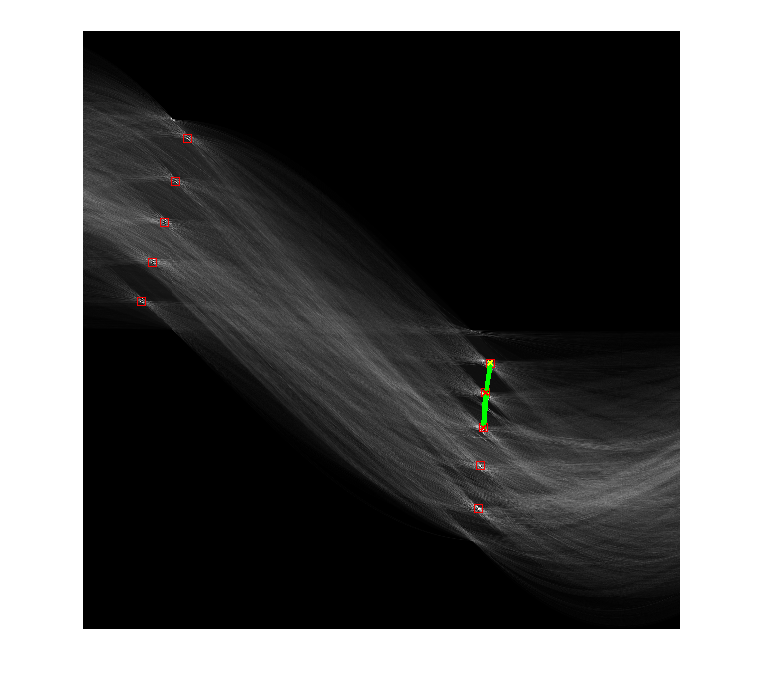
\includegraphics[scale=0.238]{fig/houghlineshough.png}
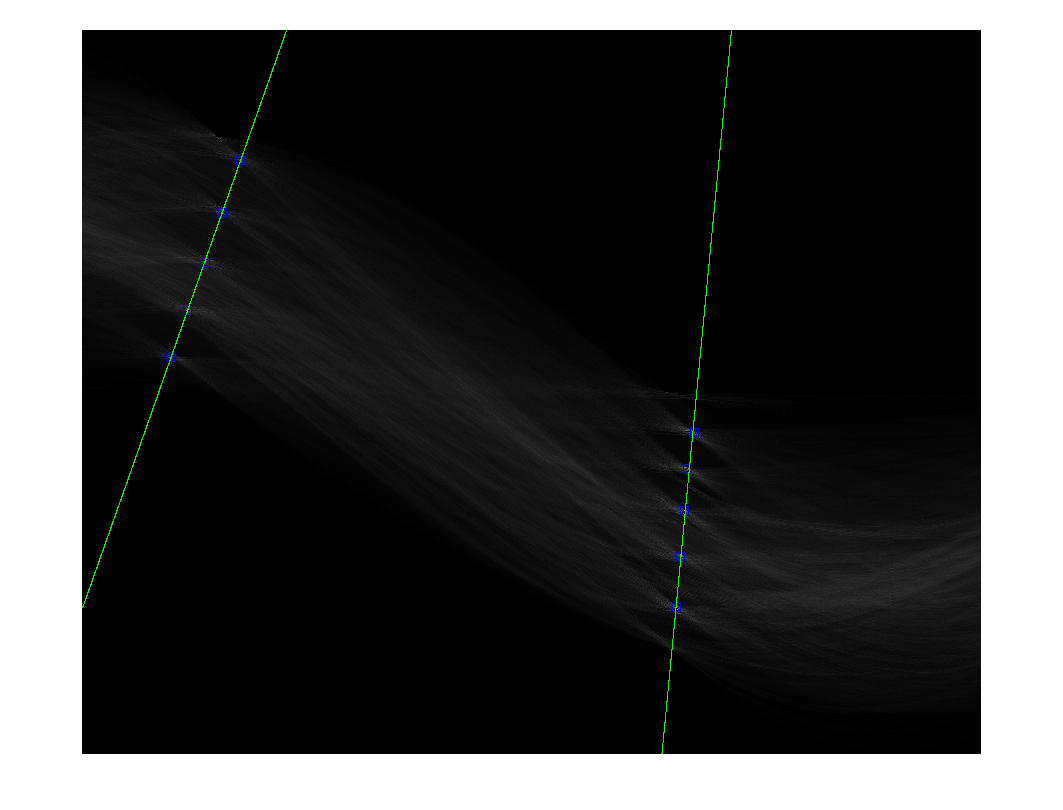
\includegraphics[scale=0.2]{fig/houghlinesRANSAC.png}
\end{center}
\caption{\label{houghlines}Détections de droites dans la transformée de Hough}
\end{figure}
\end{frame}

\begin{frame}{Raffinement du grillage}

	\begin{columns}
		\begin{column}{5cm}
		\begin{itemize}
			\item\textbf{Par colorimétrie}
			\begin{itemize}
				\item Kmeans couleur sur le grillage
			\end{itemize}
		\end{itemize}
		\end{column}

		\begin{column}{5cm}
			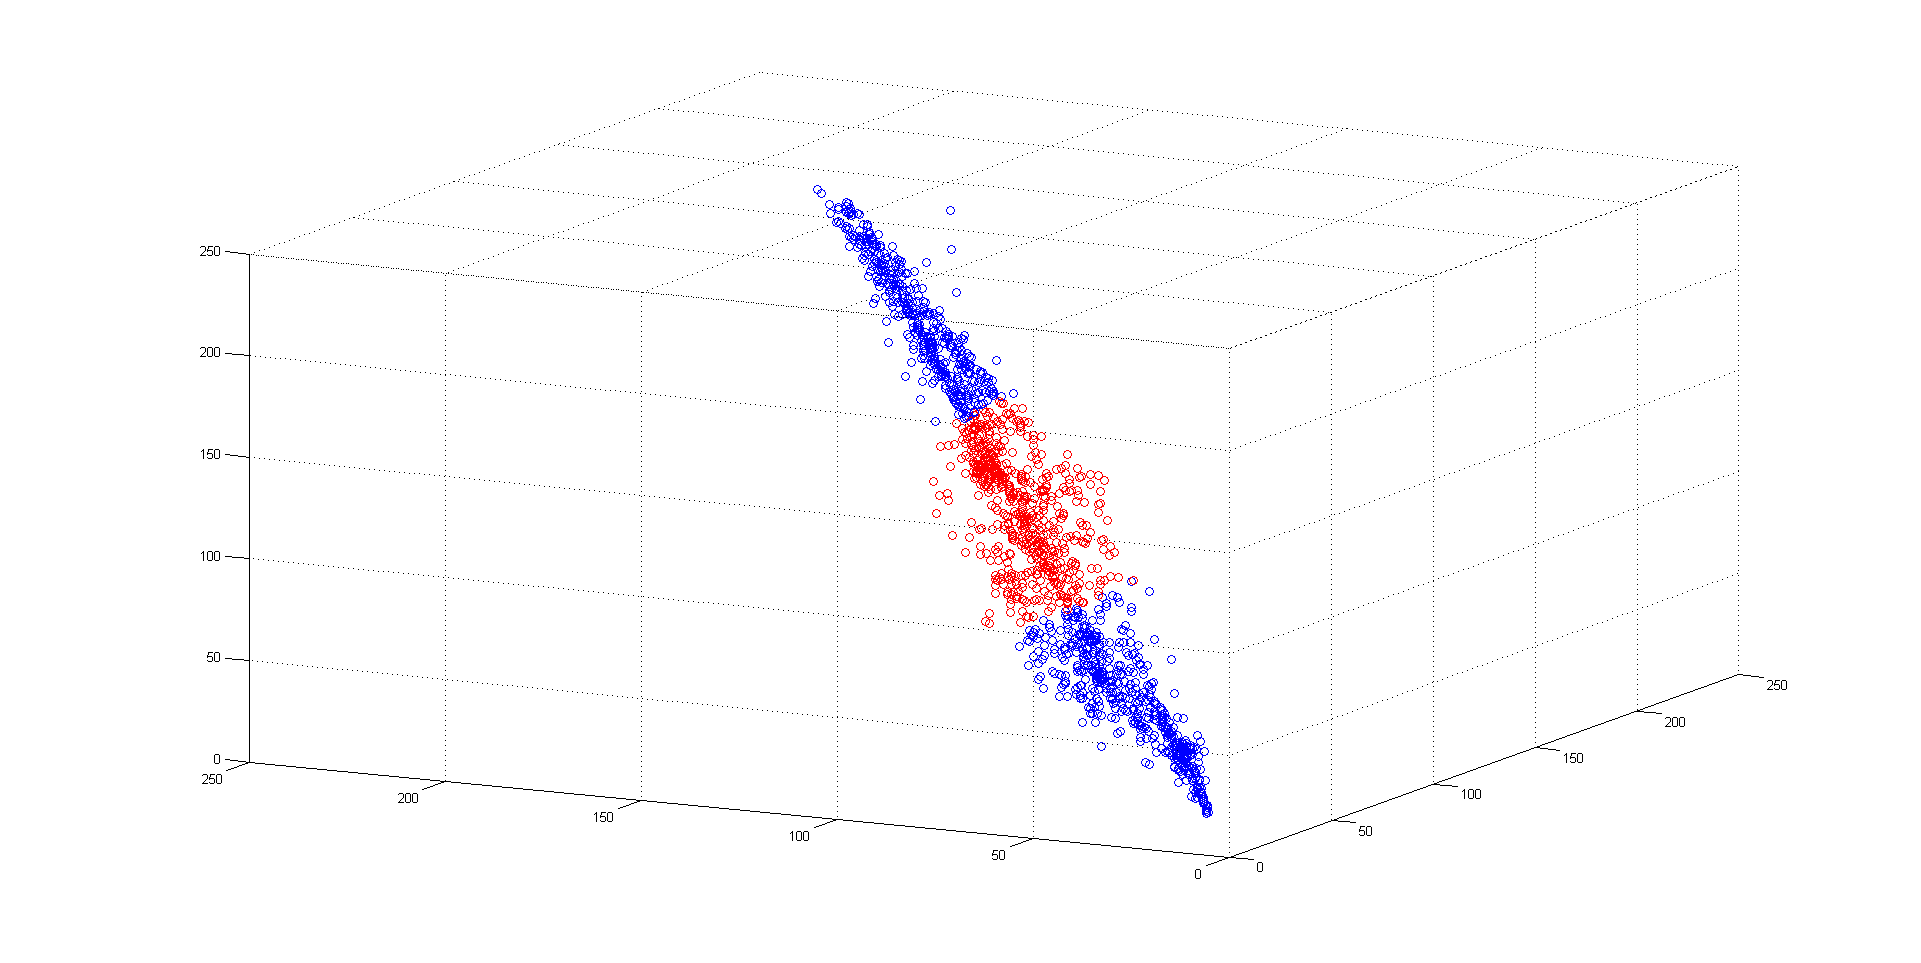
\includegraphics[width = 1 \columnwidth]{fig/Kmeans.png}
		\end{column}
	\end{columns}
	
	\begin{columns}
		\begin{column}{5cm}
		\begin{itemize}
			\item\textbf{Par périodicité dans Hough}
			\begin{itemize}
				\item Période majoritaire dans la ligne trouvée
			\end{itemize}
		\end{itemize}
		\end{column}
		\begin{column}{5cm}
	\begin{tabular}{cc}
		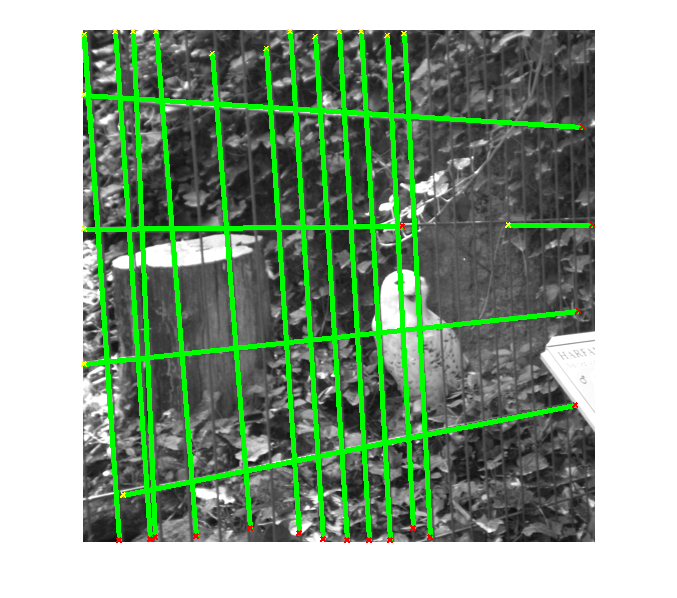
\includegraphics[width = 0.5 \columnwidth]{fig/grillagesansraf.png}
		& 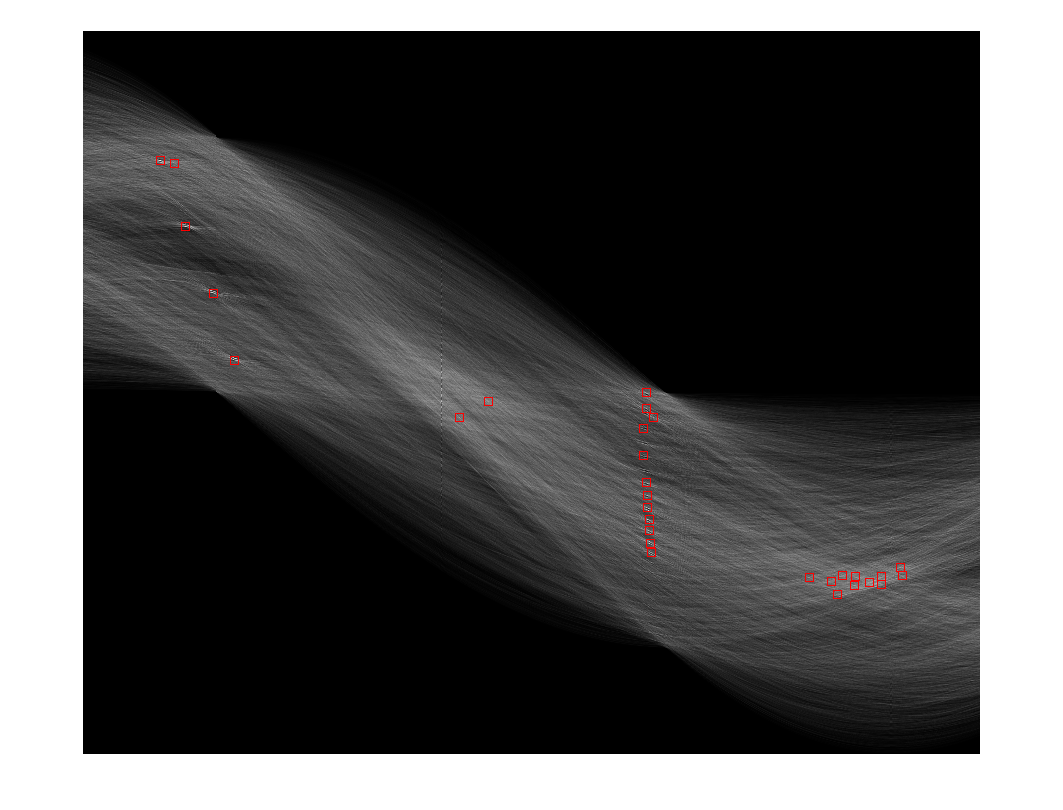
\includegraphics[width = 0.5 \columnwidth]{fig/houghsansraf.png} \\
		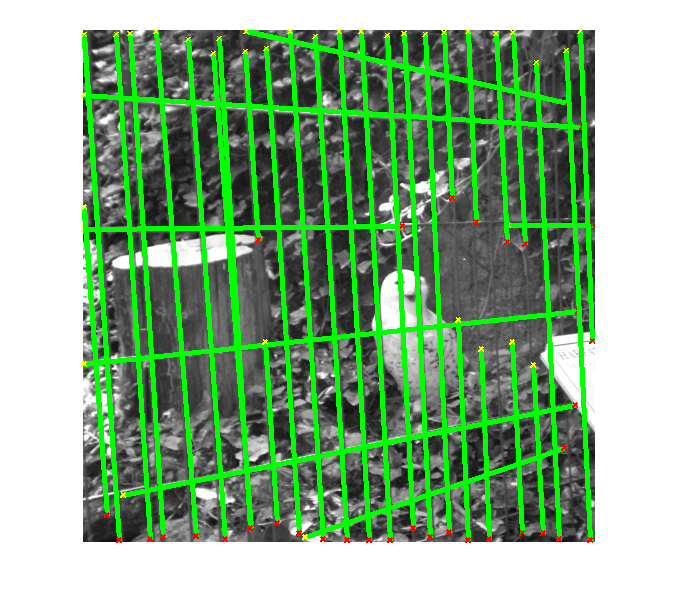
\includegraphics[width = 0.5 \columnwidth]{fig/grillageavecraf.png}
		& 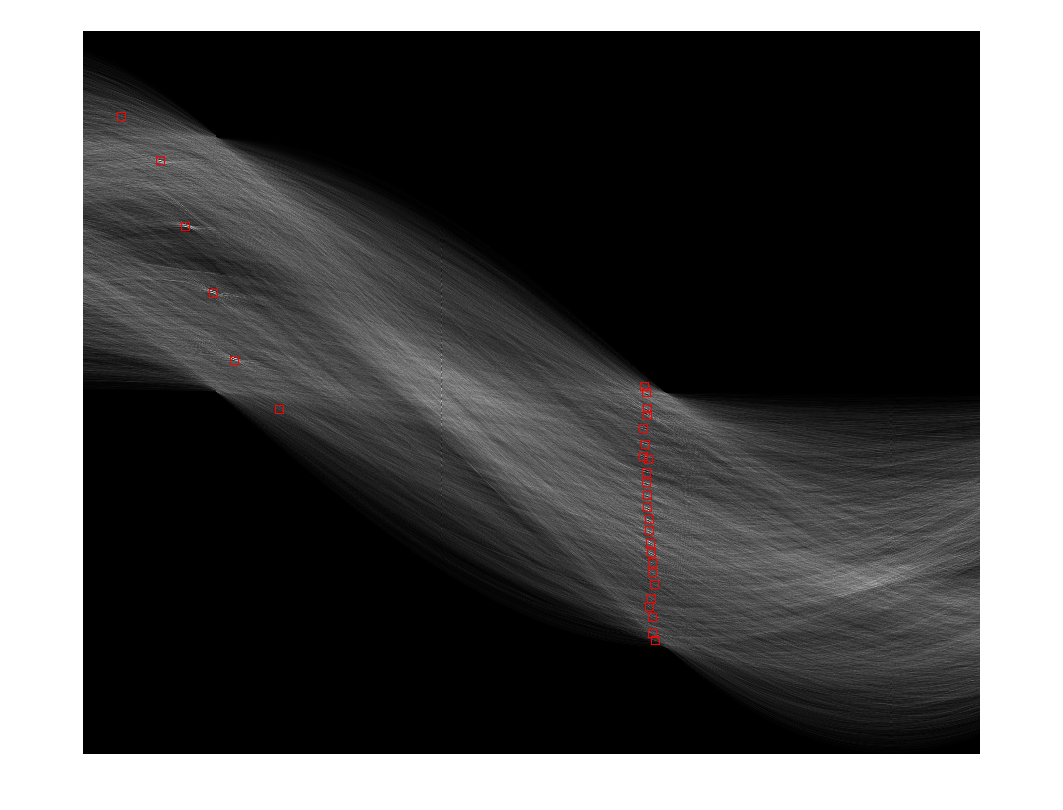
\includegraphics[width = 0.5 \columnwidth]{fig/houghavecraf.png}
	\end{tabular}		\end{column}
	\end{columns}

\end{frame}

